\section{Requerimientos funcionales}
A continuación, se presenta un listado con los requerimientos funcionales que se obtuvieron.
El listado de requerimientos funcionales se encuentra dividido de acuerdo con los módulos que se identificaron.

\paragraph{}
\begin{figure}[H]
	\centering
	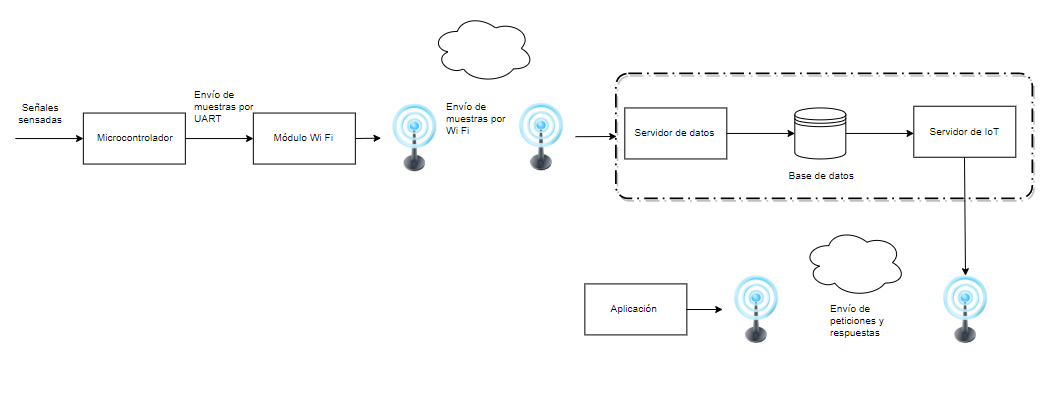
\includegraphics[scale=.3]{Capitulo3/img/diagramaBloques.png}
	\caption{Diagrama a bloques del sistema}
	\label{fig:diagrama_dispMonitoreo}
\end{figure}

\begin{itemize}
	\item Módulo de Microcontrolador.
	\item Módulo de Servidor.
	\item Módulo de Aplicación de usuario.
\end{itemize}

\paragraph{Módulo de Microcontrolador}.
%\begin{enumerate}[label=RF\arabic*]
%	\item Proporcionar un mecanismo de comunicación vía IIC desde el sensor MCP39F521 hacia el microcontrolador DSPIC30F4013.
%	\item Proporcionar un mecanismo de comunicación vía UART desde el microcontrolador DSPIC30F4013 hacia el módulo Wi-Fi MIKROE-2542.
%\end{enumerate}
\begin{longtable}{|M{1.6cm}|M{4.0cm}|M{6.0cm}|}
    \caption{Requerimientos Funcionales del Módulo de Microcontrolador}
	\hline
	\textbf{RF} & \textbf{Nombre} & \textbf{Descripción} \\ 
	\hline
 	\begin{enumerate}[label=RF\arabic*]
 	    \item.
 	\end{enumerate}
 	& Comunicación sensor-microcontrolador
 	& Proporcionar un mecanismo de comunicación vía IIC desde el sensor MCP39F521 hacia el microcontrolador DSPIC30F4013. \\
    \hline
    \begin{enumerate}[label=RF\arabic*]
        \setcounter{enumi}{1}
 	    \item.
 	\end{enumerate}
 	& Comunicación microcontrolador-módulo WiFi
 	& Proporcionar un mecanismo de comunicación vía UART desde el microcontrolador DSPIC30F4013 hacia el módulo Wi-Fi MIKROE-2542. \\
    \hline
\end{longtable}



\paragraph{Módulo de Servidor}.
%\begin{enumerate}[label=RF\arabic*.]
%	\setcounter{enumi}{2}
%	\item Proporcionar un servicio para la recepción de los paquetes enviados por el módulo Wi-Fi MIKROE-2542 y su almacenamiento en un archivo de formato de texto.
%	\item Proporcionar un servicio de comunicación vía HTTP para el envío de la información almacenada para dar respuesta a las peticiones realizadas por el usuario desde la aplicación móvil.  
%\end{enumerate}
\begin{longtable}{|M{1.6cm}|M{4.0cm}|M{6.0cm}|}
    \caption{Requerimientos Funcionales del Módulo de Servidor}
	\hline
	\textbf{RF} & \textbf{Nombre} & \textbf{Descripción} \\ 
	\hline
 	\begin{enumerate}[label=RF\arabic*]
 	    \setcounter{enumi}{2}
 	    \item.
 	\end{enumerate}
 	& Servicio para la recepción de paquetes del módulo Wi-Fi
 	& Proporcionar un servicio para la recepción de los paquetes enviados por el módulo Wi-Fi MIKROE-2542 y su almacenamiento en un archivo de formato de texto.\\
    \hline
    \begin{enumerate}[label=RF\arabic*]
        \setcounter{enumi}{3}
 	    \item.
 	\end{enumerate}
 	& Servicio de comunicación vía HTTP
 	& Proporcionar un servicio de comunicación vía HTTP para el envío de la información almacenada para dar respuesta a las peticiones realizadas por el usuario desde la aplicación móvil. \\
    \hline
\end{longtable}



\paragraph{Módulo de Aplicación de usuario}.
%\begin{enumerate}[label=RF\arabic*.]
%	\setcounter{enumi}{4}
%	\item Proporcionar un mecanismo para la vinculación entre la aplicación y el servidor.
%	\item Proporcionar un servicio de comunicación vía HTTP para la generación de peticiones al servidor.
%	\item Proporcionar un mecanismo para la visualización en tiempo real de la generación  de la energía producida por el sistema fotovoltaico.
%	\item Proporcionar un mecanismo para la generación de estadísticas de la producción de energía por el sistema fotovoltaico.
%	\item Informar por medio de notificaciones cuando el sistema fotovoltaico dejó de producir energía, así como al final del día notificar si se produjo más o menos energía que el promedio diario de producción.  
%\end{enumerate}
\begin{longtable}{|M{1.6cm}|M{4.0cm}|M{6.0cm}|}
    \caption{Requerimientos Funcionales del Módulo de Aplicación de usuario}
	\hline
	\textbf{RF} & \textbf{Nombre} & \textbf{Descripción} \\
	\hline
 	\begin{enumerate}[label=RF\arabic*]
 	    \setcounter{enumi}{4}
 	    \item.
 	\end{enumerate}
 	& Vinculación de aplicación con servidor.
 	& Proporcionar un mecanismo para la vinculación entre la aplicación de usuario y el servidor.\\
    \hline
    \begin{enumerate}[label=RF\arabic*]
        \setcounter{enumi}{5}
 	    \item.
 	\end{enumerate}
 	& Comunicación servidor-aplicación de usuario 
 	& Proporcionar un servicio de comunicación vía HTTP para la generación de peticiones al servidor. \\
    \hline
    \begin{enumerate}[label=RF\arabic*]
        \setcounter{enumi}{6}
 	    \item.
 	\end{enumerate}
 	& Monitoreo en Tiempo Real 
 	& Proporcionar un mecanismo para la visualización en tiempo real de la generación  de la energía producida por el sistema fotovoltaico. \\
    \hline
    \begin{enumerate}[label=RF\arabic*]
        \setcounter{enumi}{7}
 	    \item.
 	\end{enumerate}
 	& Estadísticas de la producción de energía 
 	& Proporcionar un mecanismo para la generación de estadísticas de la producción de energía por el sistema fotovoltaico. \\
    \hline
    \begin{enumerate}[label=RF\arabic*]
        \setcounter{enumi}{8}
 	    \item.
 	\end{enumerate}
 	& Notificaciones del Sistema fotovoltaico 
 	& Informar por medio de notificaciones cuando el sistema fotovoltaico dejó de producir energía, así como al final del día notificar si se produjo más o menos energía que el promedio diario de producción. \\
    \hline
\end{longtable}